\documentclass[11pt]{article}
\usepackage[hmargin=1in,vmargin=1in]{geometry}
\usepackage[document]{ragged2e}
\usepackage{xcolor}
\usepackage{amsmath,amssymb,amsfonts,url,sectsty,framed,tcolorbox,framed}
\usepackage{tikz}
\usepackage{nicematrix}
\newcommand{\pf}{{\bf Proof: }}
\newtheorem{theorem}{Theorem}
\newtheorem{lemma}{Lemma}
\newtheorem{proposition}{Proposition}
\newtheorem{definition}{Definition}
\newtheorem{remark}{Remark}
\newcommand{\qed}{\hfill \rule{2mm}{2mm}}


\begin{document}
%%%%%%%%%%%%%%%%%%%%%%%%%%%%%%%%%%%%%%%%%%%%%%%%%%%%%%%%%%%%%%%%%%%%%
\noindent
\rule{\textwidth}{1pt}
\begin{center}
{\bf [CS304] Introduction to Cryptography and Network Security}
\end{center}
Course Instructor: Dr. Dibyendu Roy \hfill Winter 2022-2023\\
Scribed by: Chitranshi Srivastava (202051055) \hfill Lecture 3 and 4 (Week \#2)
\\
\rule{\textwidth}{1pt}
%%%%%%%%%%%%%%%%%%%%%%%%%%%%%%%%%%%%%%%%%%%%%%%%%%%%%%%%%%%
%write here
In the previous week, we discussed about the basics of cryptography and some classical ciphering techniques. We continue from there in this week.
\section{Classical Ciphering Techniques}
\subsection{Playfair Cipher}
It is a multi-letter encryption technique in which pairs of letters are encrypted instead of single letters.\\
\textbf{Encryption : }\\
We take a 5 $\times$ 5 matrix. Each of the 25 alphabets must be unique and one letter of the alphabet (usually J) is omitted from the table as we need only 25 alphabets instead of 26. If the plaintext contains J, then it is replaced by I. Now let us see how to generate this key table using the secret key.\\


In a key table, the first characters (going left to right) in the table is the phrase, excluding the duplicate letters. The rest of the table will be filled with the remaining letters of the alphabet, in natural order.\\
\underline{Note:}
\begin{itemize}
    \item If there is an odd number of letters, a X is added to the last letter.
    \item If there are duplicates present next to each other, insert an X between the two duplicate letters.
\end{itemize}

Now let us generate the key table for the given example.\\
\textbf{Example :}\\
\textbf{Secret Key :} PLAYFAIR EXAMPLE\\
\begin{center}
    \begin{bmatrix}
    P & L & A & Y & F\\
    I & R & E & X & M\\
    B & C & D & G & H\\
    K & N & O & Q & S\\
    T & U & V & W & Z\\
\end{bmatrix}
\end{center}
\underline{\textbf{Process}}
\begin{itemize}
    \item If both the letters are in the same column, take the letter below each one (going back to the top if at the bottom)
    \item If both letters are in the same row, take the letter to the right of each one (going back to the left if at the farthest right)
    \item If neither of the preceding two rules are true, form a rectangle with the two letters and take the letters on the horizontal opposite corner of the rectangle.
\end{itemize}
We use the above rules to get the cipher text.\\
\begin{center}
    $\begin{pNiceMatrix}[margin]
    P & L & \Block[draw,fill=yellow!15,rounded-corners]{5-1}{} A & Y & F \\
    \Block[draw,fill=blue!15,rounded-corners]{2-5}{}
    I & R & E & X & M \\
    B & C & D & G & H \\
    K & N & O & Q & S \\
    T & U & V & W & Z \\
    \end{pNiceMatrix}$
\end{center}

\textbf{Plain text : } HIDE $\Rightarrow$ HI DE\\
\textbf{Cipher text : } BM OD $\Rightarrow$ BMOD\\
\textbf{Plain text : } SACHIN $\Rightarrow$ SA CH IN\\
\textbf{Cipher text : } OF DB RK $\Rightarrow$ OFDBRK\\
\textbf{Decryption :}\\
\begin{itemize}
    \item If both the letters are in the same column, take the letter above each one (going back to the bottom if at the top)
    \item If both letters are in the same row, take the letter to the left of each one (going back to the right if at the farthest left)
    \item If neither of the preceding two rules are true, form a rectangle with the two letters and take the letters on the horizontal opposite corner of the rectangle.
\end{itemize}
\textbf{Example:}\\
\textbf{Secret Key :} PLAYFAIR EXAMPLE\\
\textbf{Cipher Text :} BMOD $\Rightarrow$ BM OD\\
Since they both lie in different row and column, we form a rectangle and we use the above rules to decrypt the message.\\
\textbf{Plain text : } HI DE $\Rightarrow$ HIDE\\
\subsection{Hill Cipher}
It is a multi-letter ciphering technique in which the secret key is an n$\times$n invertible matrix.\\
\textbf{Secret Key :} A = $(a_{ij})_{n \times n}$ ,   where $a_{ij} \in Z_{26}$\\
\textbf{Plain text :} M = $m_1 m_2 m_3 m_4....m_n$\\
\textbf{Encryption :} \\
\begin{center}
    $C = A \cdot M = c_1c_2....c_n$
\end{center}
\textbf{Decryption:}\\
\begin{center}
    $M = A^{-1} \cdot C$
\end{center}
The inverse of matrix A is given as:
\begin{center}
    $A^{-1} = \frac {1}{|A|} \cdot adj(A)$
\end{center}
where $|A|$ is determinant of A and adj(A) is adjoint of matrix A.\\
\underline{Note:}
While calculating inverse of matrix A during decryption, all the calculations should be done under modulo 26.
\subsection{Substitution Cipher}
In this technique, there is a substitution from the set of alphabets to itself. It need not be a bijection. \\
S: \{A,B.....,Z\} $\rightarrow$ \{A,B.....,Z\} \\
Here, S is the secret key and Cipher text = S(Plain text)\\
The number of secret keys possible : $\#S = 26^{26} \approx 2^{122}$\\
But if the substitution is limited for bijections, then $\#S = 26!$\\
Substitution Ciphers are prone to brute force attacks and exhaustive search. Since the cipher text is known, frequency distribution analysis based on natural language can be used to break the code.
\section{Kerchoff's Principle}
It is the concept that a Cryptographic system should be designed to be secure, even if all its details, except for the key, are publicly known. It forms the basis of open security and security by design.\\
If the algorithm design is hidden, then only limited number of people will be able to use it.\\
Also, if the design is not public, then it is more prone to security vulnerabilities. Larger the number of people cryptanalyzing it, more is the probability of finding security flaws and improving the algorithm. For long term usage, those algorithms that have been published and thoroughly analyzed provide much more security.
\section{Shannon's notion of perfect secrecy}
An algorithm provides perfect secrecy if the encrypted text received using that algorithm reveals absolutely nothing about the plain text(or unencrypted text). Not even a single bit of information about the actual message is revealed by the cipher text.  \\
Suppose, we have a single but message and we are given that in the message P(0) = 0.9 and P(1) = 0.1. After encryption, if the cipher text does not reveal any additional information about guessing the message, that is, if after receiving the cipher text, the P(0) \neq (0.9 + $\epsilon), where \epsilon > 0 $, which means the probability of guessing remains the same, then the algorithm is said to provide perfect secrecy.\\
Mathematically,
\begin{center}
    $Pr[M=m|C=c] = Pr[M=m]$\\
    $Pr[message | cipher text] = Pr[message]$
\end{center}
There are certain algorithms which provide perfect secrecy with some limitations. But these limitations make these algorithms impractical. For example, One Time Padding(OTP) algorithm.
\section{Symmetric Key Cipher}
In these ciphers, the same key is used for both encryption and decryption and hence must be kept secret from everyone other than the sender and the receiver. These are of two types
\begin{itemize}
    \item Block Ciphers
    \item Stream Cipher
\end{itemize}
\subsection{Block Cipher}
The message to be encrypted is divided into fixed size blocks and these blocks are encrypted, that is, the encryption is done in block-wise manner. For example, DES algorithm can encrypt 64-bit messages. So if we have a message having 128 bits, it will be divided into 2 blocks of 64 bits and encryption would be done on each block.\\
$M = m_o||m_1||....||m_n$\\
    length of $m_i$ = l\\
One way of encryption is to encrypt each block and then concatenate the encrypted blocks in the same order.\\
\textbf{Encryption :}\\
$C = Enc(m_0, K) || Enc(m_1, K) || .... || Enc(m_n, K) = C_0 || C_1 || .... || C_n$\\
There can be some other algorithms where we can do some mixing of the blocks to generate the cipher text.\\
Both Substitution Networks and Feistal networks are type of  block ciphers
\subsection{Stream Cipher}
Here, the message is a stream of bits and encryption is done bitwise. 
$M = m_0m_1...m_l,$ where $ m_i \in {0, 1}$\\
We use an algorithm to generate another bit stream using the secret key.\\
$Z = Z_0Z_1...Z_l,$ where $ Z_i \in {0, 1}$\\
To generate the cipher text, we do XOR between bits of plain text and bits of Z.\\
\textbf{Encryption : }\\
$C = (m_0 \oplus Z_0, m_1 \oplus Z_1,...., m_l \oplus Z_l)$\\
During decryption, the same bit stream Z will be generated using the secret key and XOR will be performed with the cipher text to get the original message.\\
\textbf{\underline{Note }:} Xor function is just taken as an example. It can be another other form of computation.
\subsection{Usage of Block Ciphers and Stream Ciphers}
There are some algorithms which generate $2^{80} - 1$ bit long bit stream by taking 80 bit key as an input. Hence, using stream cipher, very long messages can be encrypted. However, this is not the case with block ciphers. Hence, to encrypt the whole message using block cipher, it will take $2^{74}$ times the time taken to encrypt one block. Hence, stream ciphers provide efficiency over block ciphers.\\
\newline
However, in our daily life, the message length is not so large and the software implementation of block cipher is very good. Hence, for more practical uses where the message length is small(like whatsapp), we prefer block ciphers.\\
Stream ciphers are used generally where the length of the message is not pre-determined or we have no idea about the length of the message. For example, voice over telephony, that is, the normal phone call uses stream ciphers as the time for which two people will communicate cannot be predicted at the starting of the call.
\newline
The hardware implementation of block ciphers is very poor as it requires a lot of gates.Hence, block ciphers are not implemented in hardware. However, all the existing stream ciphers are efficiently implemented in hardware.
\section{Product Ciphers}
A Product Cipher combines two or more transformations in a manner intending that the resulting cipher is more secure than the individual transformations. It can be better in terms of both security and efficiency over the individual function. One such cipher is a Substitution Permutation Network (SPN).
\subsection{Substitution Permutation Network (SPN)}
It is a product cipher based on a substitution box and a permutation box. Suppose we have a message of length $n \cdot r$. A substituion S and a permutation P be defined as:\\
$S: \{0, 1\}^n \rightarrow \{0, 1\}^m$\\
    $P: \{0, 1,..., m\cdot r - 1\} \rightarrow \{0, 1,..., m\cdot r - 1\} $\\
We do a substitution on r blocks of length n, which will generate a $m \cdot r$ length text. Then, performing a permutation on this $m \cdot r$ length text to get the cipher text.
\begin{center}
    \tikzset{every picture/.style={line width=0.75pt}}      
    
    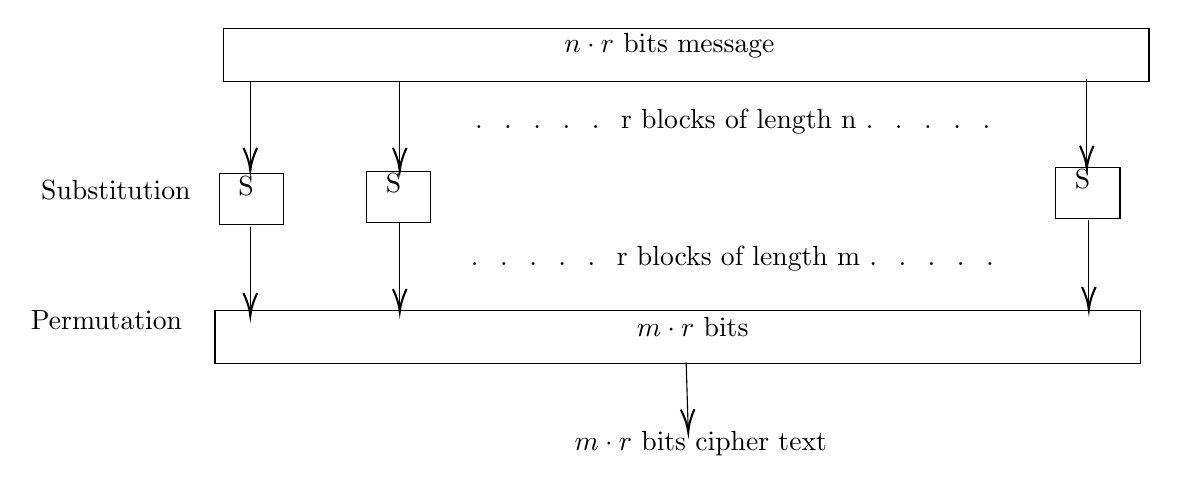
\begin{tikzpicture}[x=0.75pt,y=0.75pt,yscale=-1,xscale=1]
    \draw   (112,21) -- (558,21) -- (558,46.6) -- (112,46.6) -- cycle ;
    \draw    (125,46.6) -- (125,87.6) ;
    \draw [shift={(125,89.6)}, rotate = 270] [color={rgb, 255:red, 0; green, 0; blue, 0 }  ][line width=0.75]    (10.93,-3.29) .. controls (6.95,-1.4) and (3.31,-0.3) .. (0,0) .. controls (3.31,0.3) and (6.95,1.4) .. (10.93,3.29)   ; 
    \draw    (197,46.6) -- (197,87.6) ;
    \draw [shift={(197,89.6)}, rotate = 270] [color={rgb, 255:red, 0; green, 0; blue, 0 }  ][line width=0.75]    (10.93,-3.29) .. controls (6.95,-1.4) and (3.31,-0.3) .. (0,0) .. controls (3.31,0.3) and (6.95,1.4) .. (10.93,3.29)   ;
    \draw    (528,45.6) -- (528,86.6) ;
    \draw [shift={(528,88.6)}, rotate = 270] [color={rgb, 255:red, 0; green, 0; blue, 0 }  ][line width=0.75]    (10.93,-3.29) .. controls (6.95,-1.4) and (3.31,-0.3) .. (0,0) .. controls (3.31,0.3) and (6.95,1.4) .. (10.93,3.29)   ;
    \draw   (110,91) -- (141,91) -- (141,115.6) -- (110,115.6) -- cycle ;
    \draw   (181,90) -- (212,90) -- (212,114.6) -- (181,114.6) -- cycle ;
    \draw   (513,88) -- (544,88) -- (544,112.6) -- (513,112.6) -- cycle ;
    \draw    (125,116.6) -- (125,157.6) ;
    \draw [shift={(125,159.6)}, rotate = 270] [color={rgb, 255:red, 0; green, 0; blue, 0 }  ][line width=0.75]    (10.93,-3.29) .. controls (6.95,-1.4) and (3.31,-0.3) .. (0,0) .. controls (3.31,0.3) and (6.95,1.4) .. (10.93,3.29)   ;
    \draw    (197,114.6) -- (197,155.6) ;
    \draw [shift={(197,157.6)}, rotate = 270] [color={rgb, 255:red, 0; green, 0; blue, 0 }  ][line width=0.75]    (10.93,-3.29) .. controls (6.95,-1.4) and (3.31,-0.3) .. (0,0) .. controls (3.31,0.3) and (6.95,1.4) .. (10.93,3.29)   ; 
    \draw    (529,113.6) -- (529,154.6) ;
    \draw [shift={(529,156.6)}, rotate = 270] [color={rgb, 255:red, 0; green, 0; blue, 0 }  ][line width=0.75]    (10.93,-3.29) .. controls (6.95,-1.4) and (3.31,-0.3) .. (0,0) .. controls (3.31,0.3) and (6.95,1.4) .. (10.93,3.29)   ;
    \draw   (108,157) -- (554,157) -- (554,182.6) -- (108,182.6) -- cycle ;
    \draw    (335,182) -- (335.94,213.6) ;
    \draw [shift={(336,215.6)}, rotate = 268.3] [color={rgb, 255:red, 0; green, 0; blue, 0 }  ][line width=0.75]    (10.93,-3.29) .. controls (6.95,-1.4) and (3.31,-0.3) .. (0,0) .. controls (3.31,0.3) and (6.95,1.4) .. (10.93,3.29)   ;
    
    \draw (275,22) node [anchor=north west][inner sep=0.75pt]   [align=left] {$n \cdot r$ bits message};
    \draw (118,91) node [anchor=north west][inner sep=0.75pt]   [align=left] {S};
    \draw (189,90) node [anchor=north west][inner sep=0.75pt]   [align=left] {S};
    \draw (521,88) node [anchor=north west][inner sep=0.75pt]   [align=left] {S};
    \draw (232,59) node [anchor=north west][inner sep=0.75pt]   [align=left] {. \ . \ . \ . \ . \ r blocks of length n . \ . \ . \ . \ .};
    \draw (230,125) node [anchor=north west][inner sep=0.75pt]   [align=left] {. \ . \ . \ . \ . \ r blocks of length m . \ . \ . \ . \ .};
    \draw (23,93) node [anchor=north west][inner sep=0.75pt]   [align=left] {Substitution};
    \draw (310,159) node [anchor=north west][inner sep=0.75pt]   [align=left] {$m \cdot r$ bits};
    \draw (18,156) node [anchor=north west][inner sep=0.75pt]   [align=left] {Permutation};
    \draw (280,214) node [anchor=north west][inner sep=0.75pt]   [align=left] {$m \cdot r$ bits cipher text};
    \end{tikzpicture}
\end{center}

\section{Feistel Network}
In a Feistel network, we have an even-length message. Suppose we have a message of 2n bits, we divide it into two equal parts $L_0 and R_0 $.
\begin{center}
    P = $L_0 || R_0$.
\end{center}
$L_0$ and $R_0$ are of $n$ bits each and are calculated using right and left shifting of P by $n$ bits respectively.\\
Let K be the secret key having length $l$. \\
A fuction f, called as round function, is defined as:
\begin{center}
    $f: \{0, 1\}^n \times \{0, 1\}^l \rightarrow \{0, 1\}^n$
\end{center}
\textbf{Encryption:}\\
The diagram for encryption is given below:

\begin{center}
    \tikzset{every picture/.style={line width=0.75pt}}       
    
    \begin{tikzpicture}[x=0.75pt,y=0.75pt,yscale=-1,xscale=1]
    
    \draw   (127,51.6) -- (261,51.6) -- (261,123) -- (127,123) -- cycle ;
    \draw   (261,51.6) -- (395,51.6) -- (395,123) -- (261,123) -- cycle ;
    \draw   (129,306.6) -- (263,306.6) -- (263,378) -- (129,378) -- cycle ;
    \draw   (263,306.6) -- (397,306.6) -- (397,378) -- (263,378) -- cycle ;
    \draw   (217,151) -- (287,151) -- (287,191) -- (217,191) -- cycle ;
    \draw    (450,158.6) -- (289,158.6) ;
    \draw [shift={(287,158.6)}, rotate = 360] [color={rgb, 255:red, 0; green, 0; blue, 0 }  ][line width=0.75]    (10.93,-3.29) .. controls (6.95,-1.4) and (3.31,-0.3) .. (0,0) .. controls (3.31,0.3) and (6.95,1.4) .. (10.93,3.29)   ;
    \draw    (328,177.6) -- (290,177.98) ;
    \draw [shift={(288,178)}, rotate = 359.43] [color={rgb, 255:red, 0; green, 0; blue, 0 }  ][line width=0.75]    (10.93,-3.29) .. controls (6.95,-1.4) and (3.31,-0.3) .. (0,0) .. controls (3.31,0.3) and (6.95,1.4) .. (10.93,3.29)   ;
     
    \draw    (328.35,124.6) -- (328,177.6) -- (327.64,231.6) -- (190,231.6) -- (191.95,305.6) ;
    \draw [shift={(192,307.6)}, rotate = 268.49] [color={rgb, 255:red, 0; green, 0; blue, 0 }  ][line width=0.75]    (10.93,-3.29) .. controls (6.95,-1.4) and (3.31,-0.3) .. (0,0) .. controls (3.31,0.3) and (6.95,1.4) .. (10.93,3.29)   ;
     
    \draw    (146,124.6) -- (146,150.6) ;
    \draw [shift={(146,152.6)}, rotate = 270] [color={rgb, 255:red, 0; green, 0; blue, 0 }  ][line width=0.75]    (10.93,-3.29) .. controls (6.95,-1.4) and (3.31,-0.3) .. (0,0) .. controls (3.31,0.3) and (6.95,1.4) .. (10.93,3.29)   ;
    
    \draw   (134,167.3) .. controls (134,159.18) and (139.37,152.6) .. (146,152.6) .. controls (152.63,152.6) and (158,159.18) .. (158,167.3) .. controls (158,175.42) and (152.63,182) .. (146,182) .. controls (139.37,182) and (134,175.42) .. (134,167.3) -- cycle ; \draw   (134,167.3) -- (158,167.3) ; \draw   (146,152.6) -- (146,182) ;
    
    \draw    (217,168.6) -- (160,167.34) ;
    \draw [shift={(158,167.3)}, rotate = 1.26] [color={rgb, 255:red, 0; green, 0; blue, 0 }  ][line width=0.75]    (10.93,-3.29) .. controls (6.95,-1.4) and (3.31,-0.3) .. (0,0) .. controls (3.31,0.3) and (6.95,1.4) .. (10.93,3.29)   ;
    
    \draw    (146,182) -- (146,244.6) -- (325.01,242.74) -- (325.97,305.6) ;
    \draw [shift={(326,307.6)}, rotate = 269.13] [color={rgb, 255:red, 0; green, 0; blue, 0 }  ][line width=0.75]    (10.93,-3.29) .. controls (6.95,-1.4) and (3.31,-0.3) .. (0,0) .. controls (3.31,0.3) and (6.95,1.4) .. (10.93,3.29)   ;
    
    
    \draw (180,75) node [anchor=north west][inner sep=0.75pt]   [align=left] {$L_0$};
    \draw (316,75) node [anchor=north west][inner sep=0.75pt]   [align=left] {$R_0$};
    \draw (318,331) node [anchor=north west][inner sep=0.75pt]   [align=left] {$R_1$};
    \draw (180,327) node [anchor=north west][inner sep=0.75pt]   [align=left] {$L_1$};
    \draw (239,159) node [anchor=north west][inner sep=0.75pt]   [align=left] {$f$};
    \draw (457,148) node [anchor=north west][inner sep=0.75pt]   [align=left] {$K$};
    \draw (169,25) node [anchor=north west][inner sep=0.75pt]   [align=left] {n bits};
    \draw (302,24) node [anchor=north west][inner sep=0.75pt]   [align=left] {n bits};
    \draw (165,380) node [anchor=north west][inner sep=0.75pt]   [align=left] {n bits};
    \draw (303,380) node [anchor=north west][inner sep=0.75pt]   [align=left] {n bits};
    
    \end{tikzpicture}
\end{center}
Mathematically:
\begin{center}
    $L_1 = R_0$\\
    $R_1 = L_0 \oplus f(R_0, K)$\\
    C (cipher text) = $L_1 || R_1$
\end{center}
\textbf{Decryption:} \\
The decryption can be done as follows:
\begin{center}
    $R_0 = L_1$\\
    $L_0 \oplus f(R_0, K) = R_1$ \\
    $L_0 \oplus f(R_0, K) \oplus f(R_0, K) = R_1 \oplus f(R_0, K)$ \\
    $L_0 = R_1 \oplus f(R_0, K)$ \\
    $L_0 = R_1 \oplus f(L_1, K)$
\end{center}
Therefore, we have expressions for both $L_0$ and $R_0$ in terms of $L_1$, $R_1$ and K.\\
Diagramatically,
\begin{center}
    \tikzset{every picture/.style={line width=0.75pt}}    
    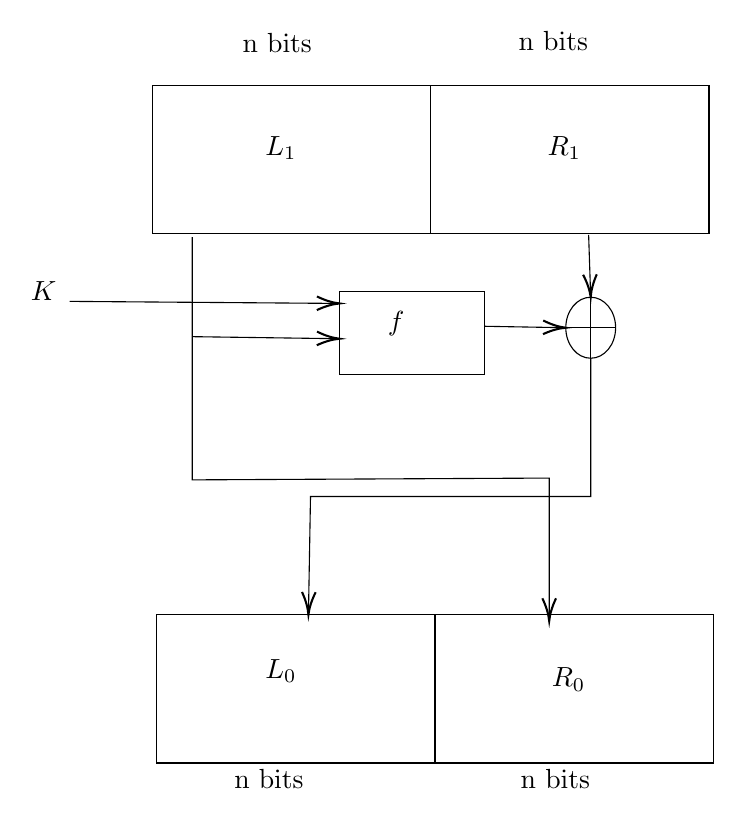
\begin{tikzpicture}[x=0.75pt,y=0.75pt,yscale=-1,xscale=1]
     
    \draw   (127,51.6) -- (261,51.6) -- (261,123) -- (127,123) -- cycle ;
    \draw   (261,51.6) -- (395,51.6) -- (395,123) -- (261,123) -- cycle ;
    \draw   (129,306.6) -- (263,306.6) -- (263,378) -- (129,378) -- cycle ;
    \draw   (263,306.6) -- (397,306.6) -- (397,378) -- (263,378) -- cycle ;
    \draw   (217,151) -- (287,151) -- (287,191) -- (217,191) -- cycle ; 
    \draw    (146,124.6) -- (146,241.6) -- (318.01,240.73) -- (318,307.6) ;
    \draw [shift={(318,309.6)}, rotate = 270] [color={rgb, 255:red, 0; green, 0; blue, 0 }  ][line width=0.75]    (10.93,-3.29) .. controls (6.95,-1.4) and (3.31,-0.3) .. (0,0) .. controls (3.31,0.3) and (6.95,1.4) .. (10.93,3.29)   ; 
    \draw   (326,168.3) .. controls (326,160.18) and (331.37,153.6) .. (338,153.6) .. controls (344.63,153.6) and (350,160.18) .. (350,168.3) .. controls (350,176.42) and (344.63,183) .. (338,183) .. controls (331.37,183) and (326,176.42) .. (326,168.3) -- cycle ; \draw   (326,168.3) -- (350,168.3) ; \draw   (338,153.6) -- (338,183) ; 
    \draw    (87,155.6) -- (215,156.58) ;
    \draw [shift={(217,156.6)}, rotate = 180.44] [color={rgb, 255:red, 0; green, 0; blue, 0 }  ][line width=0.75]    (10.93,-3.29) .. controls (6.95,-1.4) and (3.31,-0.3) .. (0,0) .. controls (3.31,0.3) and (6.95,1.4) .. (10.93,3.29)   ; 
    \draw    (146,172.6) -- (215,173.57) ;
    \draw [shift={(217,173.6)}, rotate = 180.81] [color={rgb, 255:red, 0; green, 0; blue, 0 }  ][line width=0.75]    (10.93,-3.29) .. controls (6.95,-1.4) and (3.31,-0.3) .. (0,0) .. controls (3.31,0.3) and (6.95,1.4) .. (10.93,3.29)   ;
    \draw    (287,167.6) -- (324,168.26) ;
    \draw [shift={(326,168.3)}, rotate = 181.03] [color={rgb, 255:red, 0; green, 0; blue, 0 }  ][line width=0.75]    (10.93,-3.29) .. controls (6.95,-1.4) and (3.31,-0.3) .. (0,0) .. controls (3.31,0.3) and (6.95,1.4) .. (10.93,3.29)   ; 
    \draw    (337,123.6) -- (337.93,151.6) ;
    \draw [shift={(338,153.6)}, rotate = 268.09] [color={rgb, 255:red, 0; green, 0; blue, 0 }  ][line width=0.75]    (10.93,-3.29) .. controls (6.95,-1.4) and (3.31,-0.3) .. (0,0) .. controls (3.31,0.3) and (6.95,1.4) .. (10.93,3.29)   ;
    \draw    (338,183) -- (338,249.6) -- (203,249.6) -- (202.04,304.6) ;
    \draw [shift={(202,306.6)}, rotate = 271.01] [color={rgb, 255:red, 0; green, 0; blue, 0 }  ][line width=0.75]    (10.93,-3.29) .. controls (6.95,-1.4) and (3.31,-0.3) .. (0,0) .. controls (3.31,0.3) and (6.95,1.4) .. (10.93,3.29)   ;
    
    \draw (180,75) node [anchor=north west][inner sep=0.75pt]   [align=left] {$L_1$};
    \draw (316,75) node [anchor=north west][inner sep=0.75pt]   [align=left] {$R_1$};
    \draw (318,331) node [anchor=north west][inner sep=0.75pt]   [align=left] {$R_0$};
    \draw (180,327) node [anchor=north west][inner sep=0.75pt]   [align=left] {$L_0$};
    \draw (239,159) node [anchor=north west][inner sep=0.75pt]   [align=left] {$f$};
    \draw (67,145) node [anchor=north west][inner sep=0.75pt]   [align=left] {$K$};
    \draw (169,25) node [anchor=north west][inner sep=0.75pt]   [align=left] {n bits};
    \draw (302,24) node [anchor=north west][inner sep=0.75pt]   [align=left] {n bits};
    \draw (165,380) node [anchor=north west][inner sep=0.75pt]   [align=left] {n bits};
    \draw (303,380) node [anchor=north west][inner sep=0.75pt]   [align=left] {n bits};
    \end{tikzpicture}
\end{center}
\textbf{\underline{Note} :}\\
\begin{itemize}
    \item The inverse of $f$ is not neede in the decryption process. Hence, it does not matter whether $f$ is invertible or not. So, the round function may or may not be invertible.\\
    \item It can be seen that one half of the plain text remains similar in the cipher text. However, here we have shown only one round of implementation. In actual usage, there are multiple rounds and the whole message is encrypted in later rounds.
\end{itemize}
\section{Iterated Block Cipher}
An Iterated Block Cipher is a block cipher involving the sequential repetition of an internal function (called the \textbf{Round Function}). The parameters include \textbf{the number of rounds $r$, the block size $n$ and the round keys $K_i$ of length $l$ generated from the original secret key $K$.} 
For example, we see a 3-round block cipher such that :\\
    $f \rightarrow$ Round Function\\
    $P \rightarrow$ Plain Text Block\\
    $K \rightarrow$ Secret Key\\
\begin{center}
    \tikzset{every picture/.style={line width=0.75pt}}  
    \begin{tikzpicture}[x=0.75pt,y=0.75pt,yscale=-1,xscale=1]
    \draw   (189,99) -- (259,99) -- (259,139) -- (189,139) -- cycle ;
    \draw   (313,99) -- (383,99) -- (383,139) -- (313,139) -- cycle ;
    \draw   (432,99) -- (502,99) -- (502,139) -- (432,139) -- cycle ;
    \draw    (222,180) -- (222,141) ;
    \draw [shift={(222,139)}, rotate = 90] [color={rgb, 255:red, 0; green, 0; blue, 0 }  ][line width=0.75]    (10.93,-3.29) .. controls (6.95,-1.4) and (3.31,-0.3) .. (0,0) .. controls (3.31,0.3) and (6.95,1.4) .. (10.93,3.29)   ;
    \draw    (349,179) -- (349,140) ;
    \draw [shift={(349,138)}, rotate = 90] [color={rgb, 255:red, 0; green, 0; blue, 0 }  ][line width=0.75]    (10.93,-3.29) .. controls (6.95,-1.4) and (3.31,-0.3) .. (0,0) .. controls (3.31,0.3) and (6.95,1.4) .. (10.93,3.29)   ; 
    \draw    (466,179) -- (466,140) ;
    \draw [shift={(466,138)}, rotate = 90] [color={rgb, 255:red, 0; green, 0; blue, 0 }  ][line width=0.75]    (10.93,-3.29) .. controls (6.95,-1.4) and (3.31,-0.3) .. (0,0) .. controls (3.31,0.3) and (6.95,1.4) .. (10.93,3.29)   ;
    \draw    (136,118) -- (187,118.96) ;
    \draw [shift={(189,119)}, rotate = 181.08] [color={rgb, 255:red, 0; green, 0; blue, 0 }  ][line width=0.75]    (10.93,-3.29) .. controls (6.95,-1.4) and (3.31,-0.3) .. (0,0) .. controls (3.31,0.3) and (6.95,1.4) .. (10.93,3.29)   ; 
    \draw    (260,118) -- (311,118.96) ;
    \draw [shift={(313,119)}, rotate = 181.08] [color={rgb, 255:red, 0; green, 0; blue, 0 }  ][line width=0.75]    (10.93,-3.29) .. controls (6.95,-1.4) and (3.31,-0.3) .. (0,0) .. controls (3.31,0.3) and (6.95,1.4) .. (10.93,3.29)   ;
    \draw    (383,118) -- (431,118) ;
    \draw [shift={(433,118)}, rotate = 180] [color={rgb, 255:red, 0; green, 0; blue, 0 }  ][line width=0.75]    (10.93,-3.29) .. controls (6.95,-1.4) and (3.31,-0.3) .. (0,0) .. controls (3.31,0.3) and (6.95,1.4) .. (10.93,3.29)   ;
    \draw    (503,117) -- (551,117) ;
    \draw [shift={(553,117)}, rotate = 180] [color={rgb, 255:red, 0; green, 0; blue, 0 }  ][line width=0.75]    (10.93,-3.29) .. controls (6.95,-1.4) and (3.31,-0.3) .. (0,0) .. controls (3.31,0.3) and (6.95,1.4) .. (10.93,3.29)   ;
    \draw (211,181) node [anchor=north west][inner sep=0.75pt]   [align=left] {$K_1$};
    \draw (338,180) node [anchor=north west][inner sep=0.75pt]   [align=left] {$K_2$};
    \draw (455,180) node [anchor=north west][inner sep=0.75pt]   [align=left] {$K_3$};
    \draw (214,110) node [anchor=north west][inner sep=0.75pt]   [align=left] {$f$};
    \draw (341,108) node [anchor=north west][inner sep=0.75pt]   [align=left] {$f$};
    \draw (459,109) node [anchor=north west][inner sep=0.75pt]   [align=left] {$f$};
    \draw (113,109) node [anchor=north west][inner sep=0.75pt]   [align=left] {P};
    \draw (557,107) node [anchor=north west][inner sep=0.75pt]   [align=left] {C};
    \end{tikzpicture}
\end{center}
\begin{center}
    C $\rightarrow$ cipher text\\
    $G(K) \rightarrow K_1, K_2, K_3$ (round keys)\\ 
\end{center}
The function G, which is known as the \textbf{Key Scheduling Function} takes the secret key as input generates the round keys.
\section{One Time Padding}
One Time Padding (OTP) provides perfect secrecy under some conditions.\\
\textbf{Encryption: }\\
$Enc(P, K) = P \oplus K = C$\\
where,\\
 P $\rightarrow$ Plain Text\\
    K $\rightarrow$ Secret Key\\
    $\oplus \rightarrow $ xor operation\\
\textbf{Decryption: }\\
    $Dec(C, K) = C \oplus K = P$\\
To ensure that OTP provides perfect secrecy, that is,\\
\begin{center}
    $P(message | Cipher text) = P(message)$
\end{center}
certain conditions have to be fulfilled. These are as follows :
The conditions under which OTP provides perfect secrecy are as follows:
\begin{enumerate}
    \item The secret key K cannot be used to encrypt two messages, that is, the key can not be reused.
    \item The length of key must be greater than or equal to the length of message.\\
    $length(K) \geq length(P)$
    \item Key K is uniformly selected from the key space.
\end{enumerate}
\end{document}